\subsection{Differenze tra Gradle e Maven}
Uno dei build tool più usati attualmente è senza dubbio Maven. Ci sono molte differenze tra questi due tools: flessibilità, performance, gestione delle dipendenze e molto altro. Le differenze si possono già notare dal file di configurazione, Gradle infatti ha una convenzione molto più facile e comprensibile rispetto alla tediosa configurazione del pom di Maven. Anche se entrambi usano dei metodi di miglioramento della velocità di esecuzione delle build, Gradle è senza dubbio il tool più veloce. Per essere migliore Grandle usufruisce di:
\begin{itemize}
    \item \textbf{Incrementality:} evitando il lavoro di monitoraggio dei task di I/O eseguendo solo il necessario e quando possibile processare solo i files che sono cambiati;
    \item \textbf{Build Cache:} utilizza un sistema di cache riusando gli outputs di altre build Gradle con gli stessi inputs;
    \item \textbf{Deamon:} sfrutta un long-lived process che mantiene tutte le informazioni in memoria.
\end{itemize}
Queste 3 caratteristiche rendono Gradle molto veloce, ad esempio una build Gradle con Maven verrebbe completata con un tempo 3 volte maggiore. Tutto questo è anche possibile grazie a un sistema di esecuzioni parallele di task e intra-task.
\begin{figure}[H]
\centering
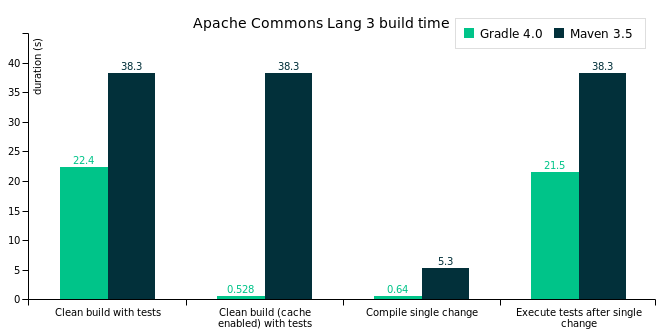
\includegraphics[width=0.7\linewidth]{0introduction/gradle/performance.png}
\end{figure}
Possiamo quindi affermare che Gradle può essere un ottimo sostituto di Maven.